\documentclass{ctexart}
\usepackage{amsmath}
\usepackage{graphicx}
\begin{document}
\title{计算物理作业 1}
\author{刘畅, PB09203226}
\maketitle

{\bf[作业1]}\quad 用Schrage方法编写随机数子程序,用连续两个随机数
作为点的坐标值绘出若干点的平面分布图; 再用$\langle x^k\rangle$测试均匀
性(取不同量级的$N$值,讨论偏差与$N$的关系)、$C(l)$ 测试其2维
独立性(总点数$N > 10^7$)。与前面的 \verb|randomz| 子程序进行比较
(采用同样的常数以及单精度或双精度实数运算),总结和评
价2个随机数产生器的随机性质量。

\section{用 Schrage 方法编写随机数发生器}
按照书上的公式
\[
az\bmod m = \begin{cases}
a(z\bmod q) - r\lfloor z/q \rfloor & \text{if } \geq 0\\
a(z\bmod q) - r\lfloor z/q \rfloor + m & \text{otherwise}
\end{cases}
\]
编程, 其中最主要的代码是 (见 \verb|schrage.c|).
\begin{verbatim}
double rand_schrage(double x)
{
    int32_t z = x * CONST_M;
    int32_t q = CONST_M / CONST_A;
    int32_t r = CONST_M % CONST_A;
    int32_t retval = CONST_A * (z % q) - r * (z / q);
    if (retval < 0)
        retval += CONST_M;
    return (double) retval / (double) CONST_M;
}
\end{verbatim}
其中的 \verb|CONST_*| 是各种常数.

将给出的 \verb|randomz| 例程转换成 C 语言, 主要的代码是 (见
\verb|randomz.c|)
\begin{verbatim}
double randomz(double x)
{
    return fmod(CONST_A * x * 1e+8, CONST_M) * 1e-8;
}
\end{verbatim}
同样, 其中的 \verb|CONST_*| 是各种常数.

\section{做  $(x_i,x_{i+1})$ 的平面分布图}
对两种随机数发生器, 取定种子值后生成 $(x_i,x_{i+1})$ 对, 打印到屏幕上.
主要代码如下, 见 \verb|generate_x_y_dataset.c|.
\begin{verbatim}
void test_rand(int nsteps, FILE *fout, double (*prand)(double))
{
    ...
    for (i = 0; i < nsteps; i++) {
        z_next = prand(z); /* generate random number */
        fprintf(fout, "%.12f\t%.12f\n", z, z_next);
        z = z_next;
    }
}
\end{verbatim}
函数声明中的 \verb|double (*prand)(double)| 是函数指针的声明方式, 这样
将比如 \verb|randomz| 作为参数传给 \verb|test_rand| 就可以生成 \verb|randomz|
的 $(x_i,x_{i+1})$ 对.

将屏幕上打印出的数据重定向到文件, 就可以用 \verb|gnuplot| 做图, 比如
\begin{verbatim}
./generate_x_y_dataset 10000 > fout
gnuplot -e "plot 'fout'; pause 10"
\end{verbatim}
见 \verb|Makefile| 文件.

首先取数据点个数为 10000, 对 \verb|randomz| 例程, 结果为:
\begin{center}
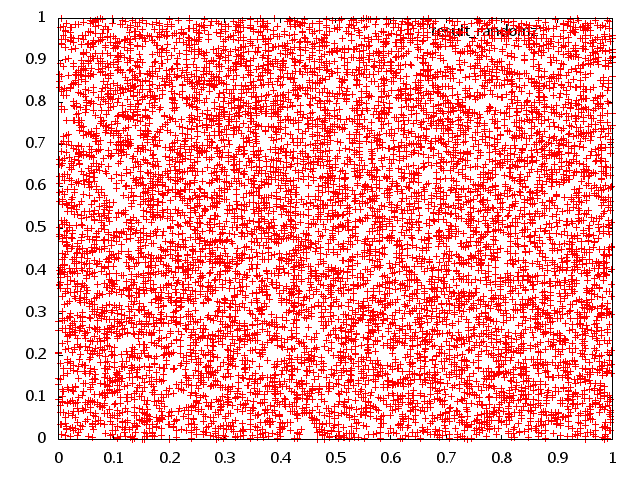
\includegraphics[width=3.5in]{../randomz_1e4.png}\\
\end{center}
对 \verb|schrage| 方法, 结果为:
\begin{center}
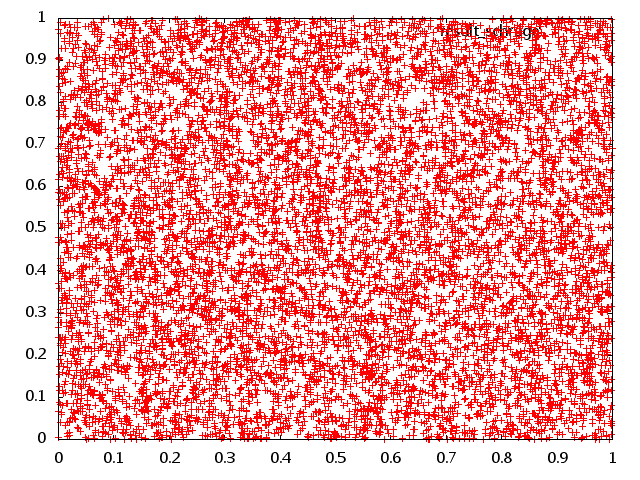
\includegraphics[width=3.5in]{../schrage_1e4.png}\\
\end{center}
然后将数据点数增加到 1000000, 对 \verb|randomz| 例程, 结果为:
\begin{center}
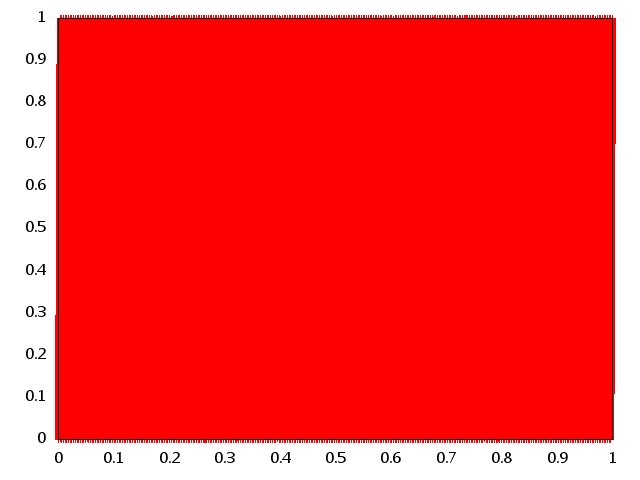
\includegraphics[width=3.5in]{../randomz_1e6.png}\\
\end{center}
\break 对 \verb|schrage| 方法, 结果为:
\begin{center}
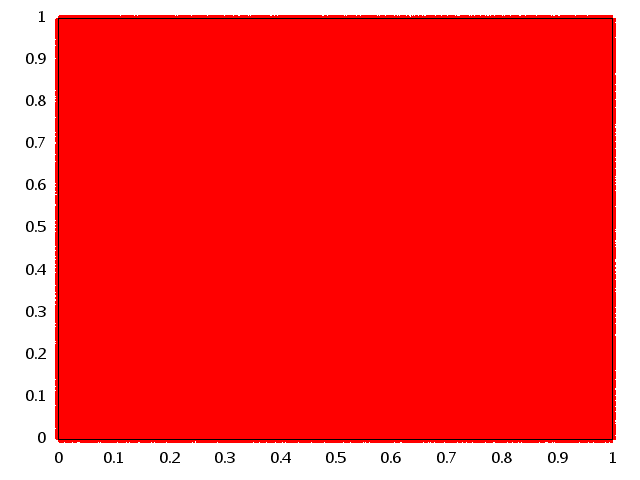
\includegraphics[width=3.5in]{../schrage_1e6.png}\\
\end{center}

可以看出对两种算法, $x_i$ 和 $x_{i+1}$ 的关联性都很弱.

\section{用 $\langle x^k \rangle$ 测试均匀性}
按照书上的公式
\begin{equation}
\langle x_n^k \rangle = \sum_{n=1} \frac{x_n^k}{N}
\end{equation}
编写计算 $\langle x^k\rangle$ 的程序, 主要代码为:
\begin{verbatim}
double test_x_k(int k, int nsteps, double (*prand)(double))
{
    ...
    accum_x_k = 0.0;
    for (i = 0; i < nsteps; i++) {
        x = prand(x);    /* generate random number */
        x_k = 1.0;       /* compute $x_i^k$ */
        for (j = 0; j < k; j++) {
            x_k *= x;
        }
        accum_x_k += x_k; /* compute $\sum_i x_i^k$ */
    }
    return accum_x_k / nsteps;
}
\end{verbatim}
详见 \verb|test_x_k_c_l.c|. 注意这个程序每次运行结果都不同.

\input ../latex_x_k_results

分析: 注意到对 $[0,1]$ 内的均匀分布, 有 $\langle x^k \rangle = \frac{1}{k+1}$,
这样 $|\langle x^k \rangle - \frac{1}{k+1}| \to 0$, 当 $n\to\infty$. 这与程序
得出的结果一致, 反映在表上竖着看每一列的值都在减小. 另外注意到每一行也有减小的规律,
这表明可能有 $\langle x^k\rangle - \frac{1}{k+1}|\to0$ 当 $k\to\infty$. 但我没法
证明这一点.

\section{计算 $C(l)$ 检验独立性}

按照书上的公式
\begin{equation}
C(l) = \frac{\langle x_n x_{n+1}\rangle - \langle x_n \rangle^2}
{\langle x_n^2 \rangle - \langle x_n\rangle ^2}
\end{equation}
计算 $C(l)$, 主要代码如下:
\begin{verbatim}
double test_c_l(int l, int nsteps, double (*prand)(double))
{
    ...
    accum_x_nl = 0.0;
    accum_x_n = 0.0;
    accum_x_n2 = 0.0;
    for (i = 0; i < nsteps; i++) {
        accum_x_nl += x * x_l;
        accum_x_n += x;
        accum_x_n2 += x*x;
        x = prand(x);
        x_l = prand(x_l);
    }
    return (accum_x_nl - accum_x_n * accum_x_n / nsteps)
           / (accum_x_n2 - accum_x_n * accum_x_n / nsteps);
}
\end{verbatim}
详见 \verb|test_x_k_c_l.c|.

\input ../latex_c_l_results

分析: 假设 $x_n$ 和 $x_{n+l}$ 独立, 这样 $\langle x_n x_{n+l} \rangle =
\langle x_n\rangle \langle x_{n+l}\rangle = \langle x_n \rangle^2$,
这样 $C(l)=0$. 程序的输出反映了这样的特性, 即随着 $N$ 增大, 计算出的 $C(l)$
减小, 直至趋于 0.

\section{比较两种算法的优劣}
从计算结果可以看出, 无论是独立性, 均匀性还是相邻两点的关联性, 两种算法都没有明显的区别.

\end{document}
